%\documentclass[]{book}
%\usepackage{graphicx}
%\usepackage{float}
%%opening
%\title{Experiments Guide}
%
%
%\begin{document}
%
%\maketitle
%
\section{Experiment 01:Motion Programming Inline Form}
Aim of the experiment
\begin{itemize}
	\item Text program execution
	\item understand PTP motion
	\item Get familiar with program creation and editing in "User" interface
\end{itemize}
Preconditions
\begin{itemize}
	\item Knowledge of how to use Navigator.
	\item Knowledge of operating modes
	\item Theoretical knowledge in motion programming (PTP type)
	\item Tool and base coordinate system calibration
\end{itemize}
Introduction
\paragraph{User programming}
Inline forms are available in the KSS for frequently used instruction. They simplify programming and facilitates user interface with controller without the need of knowing detail information about KUKA programming Language
\paragraph{Explaining Program structure}
Program structure previews a simple KRL syntax. The DEF line indicates the name of the program; this can be hidden or displayed. Declaration section after DEF-line, where variables and their data types declared.
INI - line contains the internal variables and parameters.Mind that PTP command motion is the first command in any KRL program to be fully defined. The "HOME" position is not a program specific. It is used as the first and last position. The HOME position is stored with following values in the robot controller:
\begin{figure}[H]
	
	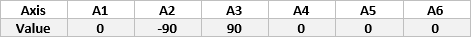
\includegraphics{ex1}
\end{figure}

\paragraph{procedure}
While in the user interface, make sure to choose the right directory KRC:R1\.click "New." to create a new module. 
Press "Select." to execute the program automatically.

\paragraph{Setting the program Override}
Program override is the velocity of the robot during Program execution. This value is specified as a percentage of the programmed velocity. Realize that in T1 mode, the maximum velocity is 250 mm/s. To modify the program override, touch the POV/HOV status indicator and slide the bar to the required value.
\paragraph{Starting Program forward (manual)}
After selecting the program, and the operating mode. Hold the enabling switch down and wait until the status bar indicates "Drives ready".
\section{Experiment 02:Motion programming Inline form}
\paragraph{Aim of the experiment}
\begin{enumerate}
	\item Understand PTP motion
	\item Get Familiar with program creation and editing in "User" interface.
\end{enumerate}
\paragraph{Preconditions}
\begin{enumerate}
	\item Familiar with Experiment 01
	\item Theoretical knowledge in motion programming (PTP type) 
\end{enumerate}
Introduction
\paragraph{Point to point motion type (PTP):}
Robot guide TCP from the current position along the fastest path to the end point specified. 
The first motion in the program must be PTP; Status and turns only defined in PTP command and ignored in CP motion.
\paragraph{"Teaching" program description:} 
"Teaching" program is an application of online robot programming using teach pendant. The robot can move in PTP motion type to the point specified by the user. The end point assigning can be applied in the different operating modes, either axis-specific or Cartesian.
\paragraph{procedure}
While in the user interface, make sure to choose the right directory KRC:R1\.Select "New." to create a new module. 
Press "Select." to execute the program automatically.
Add new motion command by pressing "Motion.". The inline form provides several settings. First, choose which kind of movement required; In this case, "PTP." is chosen. 
Next field specifies the position you want the robot to move. As a default, the first position is called "P1" and the index increments every time creating a new one. Names can be overwritten; in the program, the position called "P2."
\newpage
\paragraph{Explaining Program structure:}
As stated in "Experiment 01", the program should start by "PTP HOME  ... " and ends with the same command to ensure that all the information needed for the robot to move is fully defined. 
The next motion command is specified as PTP. Selecting "CONT." means that the end point is approximated this helps in executing next command early. In the last field, there is the name of motion data settings. It is created automatically so no need to change anything.
After setting all parameters, Robot moved to the desired position. By pressing "touch up" button position is saved.

\begin{figure}[H]
	\centering
	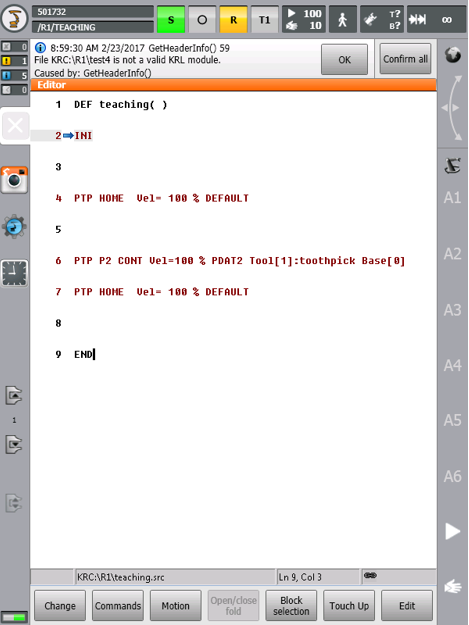
\includegraphics[scale=0.6]{ex2}
\end{figure}
\newpage
\section{Experiment 03:Motion programming (Expert level)}
\paragraph{Aim of the experiment}
\begin{enumerate}
	\item Understand and perform basic programs using KRL
	\item Get Familiar with program creation and editing in "Expert" interface
\end{enumerate}
\paragraph{Preconditions}
\begin{enumerate}
	\item Passing Experiment 02.
	\item KRL basic knowledge.
	\item Motion programming theoretical knowledge. 
	\item Tool and base coordinate system calibration
\end{enumerate}
\paragraph{Introduction}
\paragraph{Expert group}
In the Expert interface, can achieve advanced programming using the KRL programming language and perform complex application programs including subprograms, interrupt programming, loops, and program branches. 
\paragraph{"Test 3" Program Description:}
This program allows moving the robot to the HOME position using KRL commands. The program is similar to the one applied in "Experiment 01".
\paragraph{Procedure}
While in the Expert interface, make sure to choose the right directory KRC:R1\.Click "New." to create a new module. 
\begin{enumerate}
	\item In the Declaration section, HOME declared as variable, Axis-specific data type $>$ DECL AXIS HOME
	\item In the initialization section, HOME assigned be the required values $>$ HOME={AXIS: A1 90, A2 -90, A3 90, A4 0, A5 0, A6 0}
	\item The motion type selected is PTP $>$ PTP HOME
\end{enumerate}
\newpage
\begin{figure}[H]
	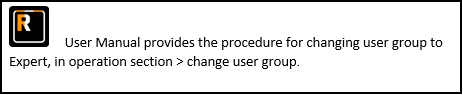
\includegraphics[scale=0.7]{Ex3}
	\centering
\end{figure}
\begin{figure}[H]
	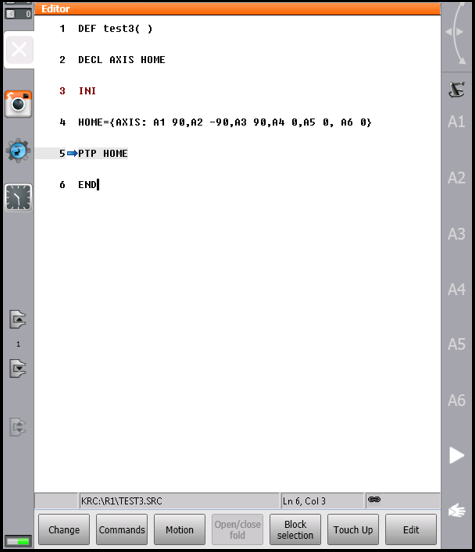
\includegraphics[scale=0.7]{Ex3_1}
	\centering
\end{figure}
\newpage
\section{Experiment 04:Motion programming (Expert level)LIN motion}
\paragraph{Aim of the experiment}
\begin{enumerate}
	\item  Understand and perform basic programs using KRL
	\item  Get Familiar with program creation and editing in "Expert" interface
	\item  Understand and implement LIN motion command
\end{enumerate}
\paragraph{Preconditions}
\begin{enumerate}
	\item  Familiar with Experiment 03
	\item  KRL basic knowledge.
	\item  Motion programming theoretical knowledge. 
	\item Tool and base coordinate system calibration.

\end{enumerate}
{Introduction}
\paragraph{LIN motion}
In the case of linear motion, the KRC "KUKA Robot Controller" calculates a straight line from the current position (the last point programmed in the program) to the point specified by the motion command. Linear motion is programmed using the keywords LIN or LIN\_REL in connection with the specification of the endpoint.
LIN motion categorized as a continuous path.
\paragraph{"test 10" Program Description}
The program moves the robot from current position to a point specified in the Cartesian way.  The path generated is linear using the LIN motion type. The program is written in KRL using the Expert user.
\begin{figure}[H]
	\centering
	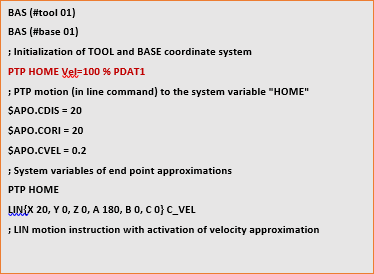
\includegraphics{Ex4}
\end{figure}
\paragraph{Procedure}
\begin{enumerate}
	\item While in the Expert interface, make sure to choose the right directory KRC:R1\.Click "New." to create a new module.
	\item In the initialization section, define the base and tool coordinate system for the robot.
	\begin{itemize}
		\item BAS(\#tool 01)
		\item BAS(\#base 01)
	\end{itemize}
		Another way for initialization is to use system variables
		\begin{itemize} 
		\item \$TOOL = TOOL\_DATA[1]
		\item \$BASE = BASE\_DATA[1]
	\end{itemize}
\item Start to assign values to end point specifications: approximation distance, approximation orientation, and approximation velocity. These specifications can be adjusted using system variables: \$APO.CDIS, \$APO.CORI, and \$APO.CVEL.
\item Add PTP command to HOME position. This is necessary in every program.
\item To generate the linear path, type LIN instruction and activate approximate positioning by inserting one of the keywords: C\_DIS, C\_ORI, and C\_VEL. at the end of the command line.

\end{enumerate}
\paragraph{Empirical Information}
In KRL program, the first motion instruction must declare a firm initial situation. Bear in mind to start any motion program with a PTP motion. PTP motion can be defined in Cartesian and axis-specific coordinates unlike CP motions (LIN and CIRC). 
HOME position is specified in axis-specific coordinate. In this program, the PTP motion written as inline form.
\begin{figure}[H]
	\centering
	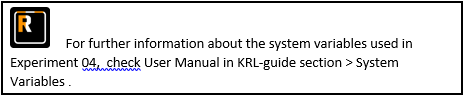
\includegraphics[scale=0.7]{Ex4_2}
\end{figure}
\begin{figure}[H]
	\centering
	\includegraphics[scale=0.7]{Ex4_3}
\end{figure}
\newpage
\section{Experiment 05:Motion programming (Expert level)PTP-POSE motion}
\paragraph{Aim of the experiment}
\begin{enumerate}
	\item  Understand and perform basic programs using  KRL
	\item  Get Familiar with program creation and editing in "Expert" interface
	\item  Understand and implement PTP motion command in Cartesian coordinate
	\item  Understand "Status and turns" concept
\end{enumerate}
\paragraph{Preconditions}
\begin{enumerate}
	\item  Passing Experiment 04
	\item  KRL basic knowledge.
	\item  Motion programming theoretical knowledge. 
	\item Tool and base coordinate system calibration.
\end{enumerate}
\paragraph{Introduction}
\paragraph{Status and Turns}

Moving the robot into a point can produce different axis positions for the same TCP (tool center point).
Referring to KRL -guide > structure type in the user manual, The entries “S” and “T”-status and turns- in a  POS structure type are used to define an unambiguous position; For this reason, it is important to start any program instruction by defining the status and turn. Since "S" and "T" not taken into consideration in the CP- motion, the first line must be complete PTP structure.
Status and Turn both require integer entries, which should be made in binary form.
\paragraph{"PTP" Program Description}
In this program, the first motion instruction is not the default HOME position- AXIS datatype variable – but instead the statement is using complete PTP instruction of type POS.
The program moves the robot to the point assigned to the HOME variable. The first motion is to the origin of base and tool system specified. Then the robot moves in linear and absolute shifts in X-axis and y –axis.
\begin{figure}[H]
	\centering
	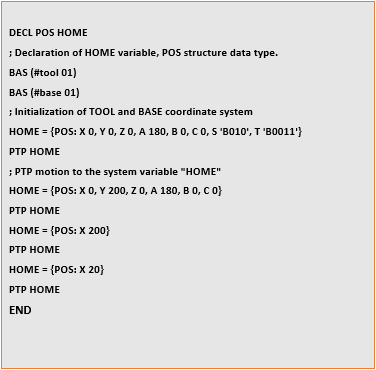
\includegraphics[scale=0.7]{Ex5_1}
\end{figure}
\paragraph{Procedure}
\begin{enumerate}
	\item While in the Expert interface, make sure to choose the right directory KRC:R1\.Click "New." to create a new module.
	\item In the initialization section, define the base and tool coordinate system for the robot.
	\begin{itemize}
	\item BAS(\#tool 01)
	\item BAS(\#base 01)
\end{itemize}
Another way for initialization is to use system variables
\begin{itemize} 
	\item \$TOOL = TOOL\_DATA[1]
	\item \$BASE = BASE\_DATA[1]
\end{itemize}
\item Write PTP motion of type POS.
\item Add PTP command to HOME position. This is necessary in every program.
\end{enumerate}
\begin{figure}[H]
	\centering
	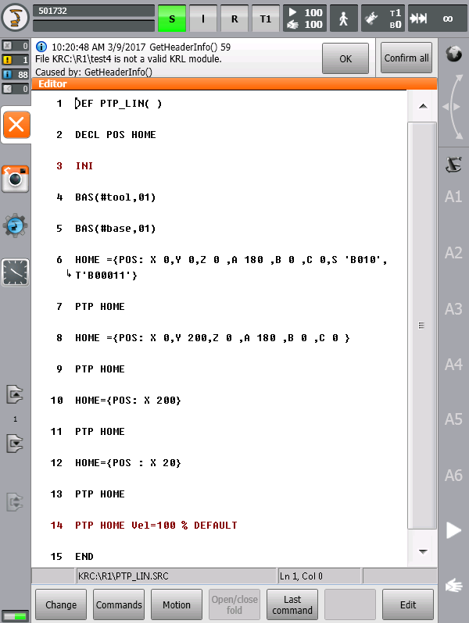
\includegraphics[scale=0.6]{Ex5_2}
\end{figure}
\section{Experiment 06:Motion programming (Expert level)Orientation Control}
\paragraph{Aim of the experiment}
\begin{enumerate}
	\item  Understand and perform basic programs using KRL
	\item  Get Familiar with program creation and editing in "Expert" interface
	\item  Understand and implement motion programming command in Cartesian coordinate with orientation control
\end{enumerate}
\paragraph{Preconditions}
\begin{enumerate}
	\item  Familiar with Experiment 05
	\item  KRL basic knowledge.
	\item  Motion programming theoretical knowledge. 
	\item  Tool and base coordinate system calibration.
\end{enumerate}
\paragraph{Introduction}
\paragraph{Orientation Control}
Defining a point in space requires three translational values beside three rotational Specifications.
A, B, C are the essential elements of KUKA KRL language. These values describe the orientations of tool in the base frame. KRL uses Euler angles (Z-Y-X) instead of fixed angles( X-Y-Z)
\paragraph{"CONE" Program Description}
In this program, the TCP changes orientation using for loop. 
\begin{figure}[H]
	\centering
	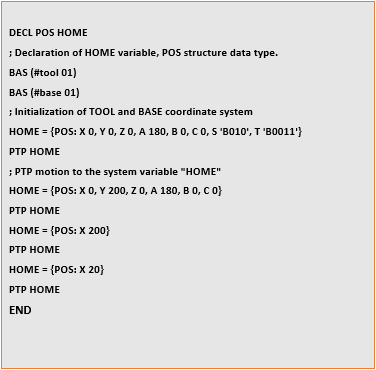
\includegraphics[scale=0.6]{Ex6_1}
\end{figure}
\begin{figure}[H]
	\centering
	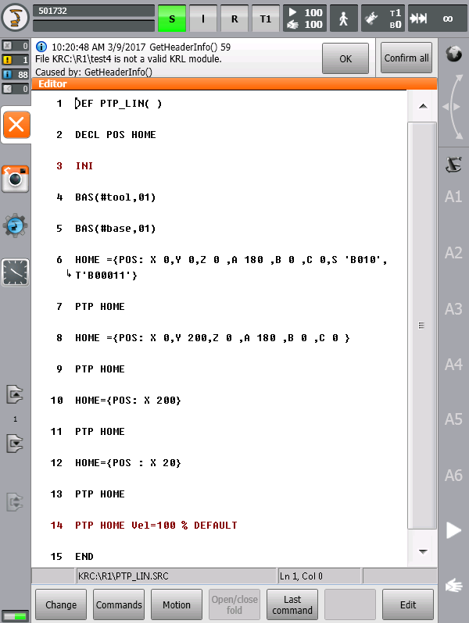
\includegraphics[scale=0.5]{Ex6_2}
\end{figure}
\section{Experiment 07:Gripper (Expert User)}
\paragraph{Aim of the experiment}
\begin{enumerate}
	\item  Understand and perform basic programs using KRL
	\item  Get Familiar with program creation and editing in "Expert" interface
	\item  Program gripper to toggle between open and close states in KRL
\end{enumerate}
\paragraph{Preconditions}
\begin{enumerate}
	\item Install gripper to the robot
	\item  KRL basic knowledge.
	\item  Air line connection AIR1. 
	\item  Tool and base coordinate system calibration.
\end{enumerate}
\newpage
\section{Experiment 08: Gripper 2 (Expert User)}

\paragraph{Aim of the experiment}
\begin{enumerate}
	\item Understand and perform programs using both Expert and Inline mode
	\item Make Modifications to inline form instructions 
	\item Use Geometric Operator 
	\item Program gripper to toggle between open and close states in KRL
\end{enumerate}

\paragraph{Precondition}
\begin{enumerate}
	\item Install gripper to the robot
	\item KRL basic knowledge.
	\item descriptionAir line connection AIR1. 
	\item Tool and base coordinate system calibration.
\end{enumerate}

This experiment is a palletizing demo, where cubes are aligned with equal spaces. Only one cube position will be taught, and the robot will automatically calculate position offsets. This is done by the geometric operator ( : ), that adsds the offset variable to the first position.
First, we need to define two variables: 
\begin{itemize}
	\item POS RR		[offset postion]
	\item INT I   		[for loop counter]
	
\end{itemize}
The X axis of RR position will be set to I in the for loop, then the robot will move to anew point consisting of the original one and the offset.
\begin{figure}[H]
	\centering
	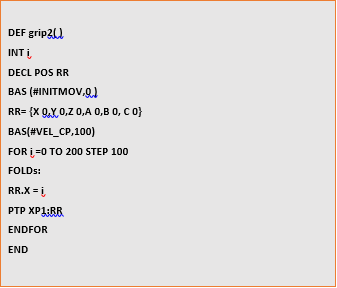
\includegraphics[scale=0.9]{Ex8}
\end{figure}
%\end{document}

